\chapter{Implementation details}
\label{sec:additional-algs}

While chapter \ref{chap:introduction-schedules} focussed more on theoretical aspects, this chapter sums up some information about the implementation. We explain why we chose C++ and Python to implement the project and present some central algorithms that were developed during this project. In addition, we provide asymptotic run times for the single algorithms.

\section{Choice or programming language(s)}
\label{sec:implementation-prog-lang}

The first question we faced was the programming language to use. We first tried to develop a prototype with Maple, because Maple already supports many mathematical concepts (in particular graph theory and probability theory) that might later be useful.

However, we quickly realized that probably Maple has some downsides for this use case: We needed something that was able to cope with quite large amount of data. While Maple might be able to do so if you are experienced enough, we went for C++, sacrificing the elegant notation of Maple, but gaining speed and control over how data are organized in memory. We also considered simple C, but quickly discarded it, because we did not want to implement some basic data structures ourselves, but instead relied on well-tested implementations (especially of Maps and Vectors). As a bonus, there are many good C++ libraries out there, some of which we made use of (Boost and GMP).

Additionally, we looked a simple language to solve several non-critical one-time tasks, such as e.g. generating a database containing all (distinct) intrees or some data analysis. We chose Python.

\section{General structure}
\label{sec:implementation-general-structure}

The algorithmic core works in two main steps: 
\begin{itemize}
\item Computing \emph{all} schedules for an intree allowed by a specific scheduling strategy.
\item Optimizing the generated schedules.
\end{itemize}

Before starting, the usual amount of command-line parsing and initialization is done, and afterwards, we can generate output files and clean up. We will now describe in short the two most important steps when generating an optimal schedule.

\subsection{Generating all schedules according to a specific strategy}
\label{sec:implementation-core-generate-schedules}

Our program basically starts off given a single intree, a certain number of processors and a scheduling strategy. According to this strategy, we then compute all initial combinations of scheduled tasks, i.e. all initial snapshots (up to equivalent snapshots).

Starting at an initial snapshot, we then recursively compute all its successors, i.e. we simulate which task finishes first and wich task shall be chosen next according to the given scheduling strategy. All of these events (task finishes, next task is chosen) are associated with a certain probability. We do this until we reach the intree containing only 1 task, which then denotes the end of the scheduling process. We thereby eliminate equivalent snapshots in order to save memory.\footnote{We also implemented a variant that does not eliminate equivalent snapshots. However, this variant quickly became too slow as the number of tasks increased. This is why we focussed on the variant that eliminates equivalent snapshots.}

After the whole snapshot DAG has been computed we can compute the expected run times of the initial snapshots (recursively, as explained in section \ref{sec:introduction-compute-expected-time-schedule}).

\subsection{Optimizing schedules}
\label{sec:implementation-core-optimizing-schedules}

Moreover, the program is capable of ``excluding the scheduler's bad choices'', i.e. it determines where the scheduler has chosen a good and where it has chosen a bad task. Then, the program discards the bad choices and leaves only the good choices, yielding a (possibly) new schedule that is optimal for a given intree.

In order to keep the program fast, we thereby had to cache quite a lot of results (since the recursions through the snapshot DAG would otherwise requiring computing the same things over and over). This, of course, leads to increased memory consumption.

\label{sec:implementation-numbers}
We implemented support for various representation of probabilities and expected run times, most notably floating point numbers. Other possible representation include doubles or rationals (through the use of e.g. the GNU Multiple Precision library).

\section{Representation of intrees and snapshots}
\label{sec:implementation-repr-intrees-snapshots}

For the representation of intrees and snapshots, we tried to find a good balance between ease of use, memory consumption and speed. We thereby rely on well-tested data structures from the C++ standard library. We now describe on a very high level how we implemented the needed data structures.

Intrees are basically maintained as a collection of edges that -- implicitly -- also store the vertices resp. tasks. We store the edges in an array such that an edge $(i,j)$ is stored as $array[i]=j$, i.e. the start of the edge is used as the array index while the target of the edge is used as the element at that particular position in the array. This is possible since we are dealing with intrees only and enables a quick lookup on which task is a successor of a given task.

Snapshots store the following things:
\begin{itemize}
\item The corresponding intree (in normalized form -- see section \ref{sec:algorithm-equivalent-snapshot}).
\item The set of currently scheduled tasks.
\item The set of its successors in the snapshot DAG and the corresponding transition probability.
\end{itemize}

Additionally, we cache many results that are frequently needed and expensive to recompute, such as the expected run time. In order to be able to reuse snapshots so that we do not recompute results for equivalent snapshots, we need some data structure that enables us to retrieve an equivalent snapshot if it already has been constructed. Therefore we introduced a pool that manages all snapshots and can be used to avoid duplicates of (equivalent) snapshots.

\newcommand{\treegeq}[1][X]{\stackrel{\text{#1}}{\geq}}

\section{Computing equivalent snapshots}
\label{sec:algorithm-equivalent-snapshot}

As mentioned in section \ref{sec:intro-first-glance-schedules}, it is possible to combine certain snapshots into one single snapshot, thereby avoiding redundant computations. The requirements for two snapshots being equivalent have been discussed there.

It is a notable fact that we can determine in polynomial time (w.r.t. the number of nodes) whether two snapshots are equivalent. This computation involves foremost a check whether the two corresponding intrees are isomorphic. 

%While it seems to be quite hard to check isomorphism for general graphs (\todo{unbedingt Referenz!}), it is feasible for intrees.

While there currently is no known algorithm that checks isomorphism in polynomial time \emph{for general graphs} (see \cite{arora2009computational}), there is a simple algorithm for isomorphism of intrees. The idea behind this algorithm is to recursively sort the predecessors of a task according to the number of their respective predecessors. An early description of a possible algorithm can be found e.g. in \cite{aho1974design}. We can easily adapt this isomorphism check to our needs in the sense that we can construct an algorithm that constructs a \emph{canonical snapshot}, and all equivalent snapshots are converted to exactly this canonical snapshot.

One thing to keep in mind is that we have to explicitly take care of the currently scheduled tasks, i.e. we have to adopt the algorithm to distinguish between scheduled and unscheduled tasks.

\subsection{The algorithm}
\label{sec:algorithm-equiv-snapshots-actual-algo}

The algorithm basically relies on an ordering of intrees (there are of course many possible, but we use a simple one). To be able to compute equivalent snapshots, this ordering has to incorporate which tasks are currently scheduled. Thus, we use an ordering that uses a set of tasks (the scheduled tasks), and does not solely rely on the structure of the intree.

\begin{definition}[Ordering of intrees with preferred tasks]
  We introduce an ordering denoted by $\treegeq$. For two intrees $I_1$ and $I_2$ and a set $X$ of tasks, we define $I_1 \treegeq I_2$ inductively. 
  \begin{itemize}
  \item If both $I_1$ and $I_2$ consist only of a root, we have $I_1 \treegeq I_2$ if and only if the root of $I_2$ is not in $X$ or the root of $I_1$ is in $X$.
  \item If the root of $I_1$ has more predecessors than the root of $I_2$, then $I_1 \treegeq I_2$.
  \item If the root of $I_1$ has the same number $r$ of predecessors as the root of $I_2$, we sort the corresponding predecessors $p_1,\dots,p_r$ resp. $q_1,\dots,q_r$ (in $I_1$ resp. $I_2$) according to $\treegeq$. Then, if $p_i \treegeq q_i \forall i\in\{1,2,\dots,r \}$, we have $I_1 \treegeq I_2$.
  \end{itemize}
\end{definition}

\todo{Examples!}

An algorithm to compute a \emph{canonical form} of a snapshot, can recursively sort the tasks in the intree according to the ordering $\treegeq$. It is shown in algorithm \ref{alg:compute-canonical-snapshot}.

\begin{algorithm}
  \begin{algorithmic}
    \Procedure{CanonicalSnapshot}{$s$} \Comment{Returns the canonical snapshot for snapshot $s$}
    \State $t \gets s.intree$ \Comment{Retrieve root of intree}
    \State $X \gets s.scheduled$ \Comment{Retrieve scheduled tasks}
    \State \textbf{return} \Call{CanonicalIntree}{$t, X$} 
    \EndProcedure
    \Statex
    \Procedure{CanonicalIntree}{$t, X$}\Comment{$t$: a (sub)tree, $X$: set of scheduled tasks}
    \State $r \gets t.root$ \Comment{Retrieve root of subtree}
    \State $CanonicalPredecessors \gets 
           \left\{ \Call{CanonicalIntree}{c, X} \mid c \in r.predecessors \right\}$
    \State \textbf{return} root with predecessors in $CanonicalPredecessors$ in sorted order according to $\treegeq$
    \EndProcedure
    \Statex
  \end{algorithmic}
  \caption{Computing canonical snapshots for a snapshot $s$ containing the corresponding intree and the tasks that are currently scheduled (as defined in section \ref{sec:processing-an-intree-of-tasks}).\todo{Algorithmus verbessern.}}
  \label{alg:compute-canonical-snapshot}
\end{algorithm}

Algorithm \ref{alg:compute-canonical-snapshot} is good for visualizing how the algorithm works. One disadvantage, however, is that recursively comparing two subtrees can be expensive. Nonetheless, there is a modification of this algorithm, that is more along the lines of \cite{aho1974design} and has a slightly better asymptotic run time. It is shown in algorithm \ref{sec:algorithm-canonical-intree-o-n}.

\begin{algorithm}
  \begin{algorithmic}[5]
    \Procedure{CanonicalIntree}{$I$, $X$}
      \State $L \gets $ number of levels in $I$
      \State Label all leaves with ``0'' if they are not in $X$, otherwise with ``1''
      \For{$i=L-2 \dots 0$}
        \For{Each non-leaf $t$ in level $i$ with predecessors $p_1,\dots,p_r$}
        \label{alg:canonical-intree-inner-loop}
          \State Label $t$ by a $(label(p_1),\dots,label(p_r))$ \Comment{Concatenate \emph{sorted} labels of predecessors}
          \label{alg:canonical-intree-concatenate-line}
        \EndFor
        \State{Sort tasks on level $i$ according to their label}
        \label{alg:canonical-intree-sorting-line}
        \State{Replace labels for tasks on level $i$ by integers $geq 1$ such that same labels obtain same numbers}
        \label{alg:canonical-intree-numbering-line}
      \EndFor
    \EndProcedure
  \end{algorithmic}
  \caption{Computing a canonical intree with a better asymptotic run time}
  \label{sec:algorithm-canonical-intree-o-n}
\end{algorithm}

Algorithm \ref{sec:algorithm-canonical-intree-o-n} is a very high level description that requires some explanations:

\begin{itemize}
\item For this algorithm, it is convenient to have a canonical intree structure in which each task directly knows its predecessors. We can transform our representation (as explained in section \ref{sec:implementation-repr-intrees-snapshots}) into this one in $O(n)$.
\item Concatenating two labels can be done in $O(1)$ (either amortized by e.g. using dynamic arrays or simply using linked lists with some additional information such e.g. a pointer to the last node in the list). Thus, the overal costs arising from line \ref{alg:canonical-intree-concatenate-line} (resp. for the whole inner loop) are $O(n)$ because the label of each task is subject to concatenation at most once. Moreover, note that the predecessors $p_1,\dots,p_r$ are sorted (they have been sorted in the previous iteration of the loop).
\item Line \ref{alg:canonical-intree-numbering-line} ensures that the labels of tasks do not become very long. To be precise, if level $i$ has exactly $l_i$ tasks, the labels for level $i$ are at most the numbers 0 to $l_1$.
\item Line \ref{alg:canonical-intree-sorting-line} from algorithm \ref{sec:algorithm-canonical-intree-o-n} shall sort in the following way: Shorter labels come first, and if two labels have the same length, they are compared lexicographically. This sorting can be implemented in $O(l_{i+1}\cdot\log l_{i+1})$, where $i$ denotes the index from the algorithm (i.e. the current level number) and $l_i$ denotes the number of tasks of $I$ on level $i$. This can be explained as follows:
  \begin{itemize}
  %\item First, we use a simple bucketsort to group the strings into buckets according to their lengths (can be done in $(O(l_{i+1}))$ if we store the lengths appropriately).
  \item We use radix sort to sort the tasks according to their labels. The labels for the $l_i$ tasks on level $i$ are composed of the labels on level $i+1$.
  %\item Each bucket is then sorted using radix sort. Assume that a bucket $j$ contains $n_j$ labels of length $j$. Then, radix sort can sort in time $O(n_j \cdot j)$.
  \item Inductively, the labels on level $i+1$ are at most the numbers 0 to $l_{i+1}$ (because there are $l_{i+1}$ tasks on level $i+1$ and there might be leaves on that level), thus requiring $O(\log l_{i+1})$ bits per label.
  %\item Thus, bucket $j$ can be radix-sorted in $O(n_j \cdot \log l_{i+1})$.
  \item Since we concatenate labels from level $i+1$ (or simply assign them label 0) to obtain the new labels on level $i$, we have $l_i$ labels of total length at most $l_{i+1}\cdot \log(\l_{i+1})$.
  \item Now, we use a modified radix sort: We first distribute the labels according to their labels into different buckets (can be done in $O(1)$ per label if we e.g. store its length appropriately). 
    %We now sort each bucket by an ordinary radix sort. Assume bucket $j$ contains $n_j$ labels of length $j$. Then, this bucket can be radix-sorted in $O(n_j \cdot j)$. 
    We can now radix-sort each bucket. Since each digit of each label of a label is examined \emph{exactly once}, we can sort all labels in $O(l_{i+1}\cdot \log l_{i+1})$ (since this is the total length of all labels on level $i$).
    %Denote the number of buckets by $B$ (obviously, $B\leq \log(l_{i+1} + 1)$). This means that all buckets can be sorted in $\sum_{j=1}^{\log(l_{i+1}+1)} O(n_j\cdot j)$.
  %\item that the whole level can be sorted in $\sum_{j=0}^B O(n_j \cdot \log l_{i+1}) = O(l_{i+1} \cdot \log l_{i+1})$.
  \item The tree can be sorted top-down in $\sum_{i=0}^{L-2}O(l_{i+1} \cdot \log l_{i+1})=O(n\cdot \log n)$.
  \end{itemize}
\item Replacing labels can be done in $O(n)$ in total since each tasks gets assigned a label only once.
\end{itemize}

\begin{theorem}
  The canonical intree of an intree with $n$ tasks can be constructed in $O(n\cdot \log n)$.
\end{theorem}

\begin{proof}
  See considerations above.
\end{proof}

\emph{Remark:} This algorithm is sometimes said to have runtime $O(n)$ -- assuming that we can express labels as integers and ignoring the fact that the total length of a label is $\log(l_{i+1})$ bits. This is, especially in the case we are considering, a very reasonable assumption because an integer nowadays has at least 32 bit, meaning that the length of a label (i.e. an integer) is only exceeded if a level of the intree contains more than $2^{32}$ tasks.

\subsection{Additional approaches}
\label{sec:algorithm-canonical-snap-additional-approaches}

We experienced that computing canonical snapshots has a major impact on the overal performance of our program, which is why we tried other approaches to tackle this problem. For completeness, we will explain them shortly. Unfortunately, they did not work out as good as expected, but maybe they are helpful for future work. In this section, we focus on the part concerning the computation of \emph{canonical intrees} (i.e. we do not distinguish between scheduled and non-scheuled leaves).

\begin{description}
\item[Tree sequence] As we have seen in previous chapters, we can describe intrees as a sequence of tasks $(x_1,\dots,x_n)$ such that task $i$ is a requirement for task $x_i$ (see section \ref{sec:foundations-graph-theory}). It is clear that we can assume certain facts about these sequences: We could e.g. assume that w.l.o.g. the sequence $(x_1,\dots,x_n)$ is non-decreasing (simply assign number by a breadth first search started by task 0). We tried to exploit the knowledge about tree sequences.

Most of the time, we are generating a certain subtree from a tree whose tree sequence is already known. We then want to know the canonical intree of this subtree. We tried exploiting the fact that we already could \emph{start} with a canonical intree. That is, we tried to construct the tree sequence of a canonical subtree by just examining the tree sequence of the original intree. 

It seems that we can compute the tree sequence of an intree $I\setminus \left\{ t \right\}$ (where $t$ is a leaf of the intree $I$) in some cases by simply removing the corresponding entry in the tree sequence. But iterating this (i.e. removing two or more tasks one after another) often leads to problems.

We could not devise a simple pattern that works as a general rule. The problem for this approach is that -- even if it might work for pure intrees -- it seems to be very complex to incorporate the fact that isomorphic intrees with a different set of scheduled tasks might or might not yield equivalent snapshots. Consider e.g. the intree $(0,0,0,1,1,2,2,3,3)$ with tasks 4, 6 and 8 scheduled (shown in figure \ref{fig:tree-sequence-not-working}). For the situation shown, it does not matter which task is the first to finish --- each resulting snapshot is equivalent to all others. However, the tree sequences obtained by removing the respective tasks are $(0,0,0,1,2,2,3,3)$, $(0,0,0,1,1,2,3,3)$ and $(0,0,0,1,1,2,2,3)$.

\begin{figure}[ht]
  \centering
  \begin{tikzpicture}[scale=.2]
    \node[circle, scale=0.75, fill] (tid0) at (4.5,1.5){};
    \node[circle, scale=0.75, fill] (tid1) at (1.5,3){};
    \node[circle, scale=0.75, fill] (tid4) at (0.75,4.5){};
    \node[circle, scale=0.75, fill, task_scheduled] (tid5) at (2.25,4.5){};
    \draw[](tid1) -- (tid4);
    \draw[](tid1) -- (tid5);
    \node[circle, scale=0.75, fill] (tid2) at (4.5,3){};
    \node[circle, scale=0.75, fill] (tid6) at (3.75,4.5){};
    \node[circle, scale=0.75, fill, task_scheduled] (tid7) at (5.25,4.5){};
    \draw[](tid2) -- (tid6);
    \draw[](tid2) -- (tid7);
    \node[circle, scale=0.75, fill] (tid3) at (7.5,3){};
    \node[circle, scale=0.75, fill] (tid8) at (6.75,4.5){};
    \node[circle, scale=0.75, fill, task_scheduled] (tid9) at (8.25,4.5){};
    \draw[](tid3) -- (tid8);
    \draw[](tid3) -- (tid9);
    \draw[](tid0) -- (tid1);
    \draw[](tid0) -- (tid2);
    \draw[](tid0) -- (tid3);
  \end{tikzpicture}
  \caption{The tree sequences for the snapshots resulting when one task finishes are different, but the snapshots are still equivalent.}
  \label{fig:tree-sequence-not-working}
\end{figure}

\item[Matula numbers] Intrees and their encodings have of course already been subject to research. One example is \cite{matula1968natural}, where a (more or less) natural bijection between intrees and natural numbers, the so-called \emph{Matula numbers}, is shown.

These numbering is inductively defined as follows: A single leaf (resp. a tree consisting of a single root) obtains the number 1. A root with predecessors $t_1,\dots,t_r$ with corresponding numbers $n_1,\dots,n_r$ obtains the number $\prod_{i=1}^r p(n_i) = p(n_1)\cdot p(n_2) \cdot \dots \cdot p(n_r)$, where $p(x)$ denotes the $x$-th prime number. See figure \ref{fig:matula-illustration} for an example.

\begin{figure}[t]
  \centering
  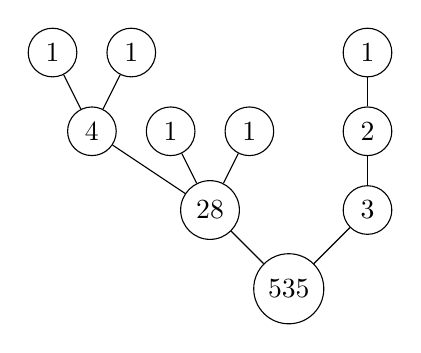
\begin{tikzpicture}
    \node[draw, circle](1_1) at (0,0){1};
    \node[draw, circle](1_2) at (1,0){1};
    \node[draw, circle](1_3) at (4,0){1};
    
    \node[draw, circle](4_1) at (.5,-1){4};
    \node[draw, circle](1_4) at (1.5,-1){1};
    \node[draw, circle](1_5) at (2.5,-1){1};
    \node[draw, circle](2_1) at (4,-1){2};

    \node[draw, circle](28_1) at (2,-2){28};
    \node[draw, circle](3_1) at (4,-2){3};

    \node[draw, circle](535) at (3, -3){535};

    \draw(1_1)--(4_1);
    \draw(1_2)--(4_1);
    \draw(1_3)--(2_1);
    \draw(1_4)--(28_1);
    \draw(1_5)--(28_1);
    \draw(4_1)--(28_1);
    \draw(2_1)--(3_1);
    \draw(28_1)--(535);
    \draw(3_1)--(535);
  \end{tikzpicture}
  \caption{A tree whose vertices are labelled by the corresponding matula numbers. Consider e.g. the node 4, whose predecessors are two nodes labelled 1. Thus, we can compute $4=p(1)\cdot p(1)$. The node labelled 28 can be computed by $28 = p(4)\cdot p(1) \cdot p(1) = 2\cdot 2 \cdot 7$. The node 535 obtains its label by $535=p(28)\cdot p(3) = 107\cdot 5$.}
  \label{fig:matula-illustration}
\end{figure}

While this description could lead to very elegant algorithms in a theoretical setting, it does not come in handy in practice because the matula numbers can be very big (more than 32 bit needed for matula numbers of 15-node intrees): As shown in \cite{onmatulanumbers}, the largest Matula number for an intree with $n\geq 5$ tasks is $p^{(n-4)}(8)$, where
\begin{eqnarray*}
  p^{(0)} (x) &=& x, \\
  p^{i}(x) &=& p\left(p^{i-1}(x)\right).
\end{eqnarray*}

The growth of $p^{n-4}(3)$ is immense as $n$ increases. We can see from table \ref{tab:certain-values-pn-2-3-growth} that for intrees with 14 tasks, we exceed the size of a 32-bit unsigned integer, and for intrees with 20 tasks, the largest corresponding matula number even exceeds a 64-bit integer (table \ref{tab:certain-values-pn-2-3-growth} shows the values of $p^{(n-4)}(8)$ for $n$ up to 20 --- if these values were too large, we restricted ourselves to the logarithm (base 2) of the respective values to determine how many bits are needed).

\begin{table}[th]
  \centering
  \begin{tabular}[ht]{cr}
    $n$ & $p^{(n-4)}(8)$ \\
    \hline
    5 & 19 \\
    6 & 67 \\
    7 & 331 \\
    8 & 2221 \\
    9 & 19577 \\
    10 & 219613 \\
    11 & 3042161 \\
    12 & 50729129 \\
  \end{tabular}
  \quad
  \begin{tabular}[ht]{crl}
    $n$ & $p^{(n-4)}(8)$ & $\log_2\left( p^{(n-4)}(8) \right)$ \\
    \hline13 & 997525853 & $<30$\\
    14 & 22742734291 & $>34$ \\
    15 & $\approx 5.92852 \cdot 10^{11}$ & $> 39$ \\
    16 & n.a. & $> 43$ \\
    17 & n.a. & $> 49$ \\
    18 & n.a. & $> 54$ \\
    19 & n.a. & $> 59$ \\
    20 & n.a. & $> 65$ \\
  \end{tabular}
  \caption{Values of $p^{(n-2)}(3)$ for certain values of $n$.}
  \label{tab:certain-values-pn-2-3-growth}
\end{table}

Note that even intrees with fewer than 20 tasks can have matula numbers greater than $p^{(20-4)}(8)$, thus even worsening the scenario. 

In addition to the huge numbers that would need to be multiplied, computing matula numbers efficiently would require us to quickly compute $p(n)$. This would probably best acchieved using a lookup table, but this would require a huge amount of memory.

\end{description}

\section{Computing all schedules according to a specific scheduling strategy}
\label{sec:implementation-computing-all-schedules}

We have seen how we can compute equivalent snapshots resp. a canonical representation of a snapshot. We now describe in short how this can be used to generate all schedules according to a specific scheduling policy.

The program starts out with a given intree and the scheduler generates a list of possible initial settings describing which tasks shall be chosen. This gives us a list of \emph{initial snapshots} where each snapshot contains the original intree and a set of tasks that shall be scheduled initially. We then process one initial snapshot after another. We describe now what we have to do for each initial snapshot.

When we have a snapshot with a certain set of scheduled tasks, the program computes the intrees that occur if one of the tasks finishes. This has to be done for every currently scheduled task. That means, that for every currently scheduled task that could finish, we obtain a new intree \emph{and} also a set of tasks that are scheduled (since we are considering non-preemtive scheduling, we have to keep the other tasks scheduled).

For each of the newly generated intrees, the scheduler determines which task shall be chosen with which probability in the next step, and generates new snapshots this way. The original snapshot stores pointers to the newly generated snapshots, associated with the respective probabilities of reaching them.

However, as aforementioned, it is useful to compute a canonical version of each snapshot, thereby eliminating quite a large amount of snapshots for which we would -- essentially -- compute the same things twice. This requires us to manage a \emph{snapshot pool} where we store all snapshots that we have encountered up to now. If a newly generated snapshot is already is in this pool, we do not continue computations on this newly generated snapshot but instead re-use the original one.

This, on the other hand, requires us to quickly find out whether a snapshot has already been generated or not (and also to retrieve its address in memory). There are several ways to acchieve this. We are using a technique that maps snapshots onto the respective addresses. We therefore basically encode the snapshot's intree and the scheduled tasks as a sequence of bits. We could do this using ordinary \texttt{int}s or \texttt{long}s (or their \texttt{unsigned} equivalents in C++), but we decided to encode them using C++'s \texttt{vector<unsigned char>}s in connection with a list of the currently scheduled tasks.

We went for this solution for several reasons:

\begin{itemize}
\item The number of intrees grows rapidly, thus quickly exceeding the range of a (32-bit) integer \cite{oeisrootedtrees}.
\item An encoding of intrees as integers in a way such that we do \emph{not} ``waste'' some encodings may be very cumbersome to implement (we could use the aforementioned Matula numbers, but as said, these are not very handy in practice --- see table \ref{tab:certain-values-pn-2-3-growth}).
\end{itemize}

Using a \texttt{vector} of course increases memory consumption compared to e.g. using an ordinary \texttt{long} but is much more convenient when it comes to implementation details and -- at least in theory -- provides a much larger range that a single \texttt{int} or \texttt{long}.

We basically describe the current intree storing the same notation as shown in this work (just stored in a \texttt{vector} of \texttt{unsigned char}s). Of course, there are more memory-efficient solutions, but since we did never experience any problems regarding memory, we went for this solution.

As mentioned in section \ref{sec:intro-computing-optimal-schedule} we have $O\left(|\left\{ T \mid T\subseteq I \right\}|\cdot n^p\right)$ snapshots for an intree with $n$ tasks scheduled on $p$ processors. We can simply call this $O\left(|D|\right)$ where $D$ denotes the snapshot DAG for a certain scheduler. Since we compute the \emph{canonical snapshot} for each of those snapshots and the run time to compute the canonical snapshot is $O(n \log n)$, we can deduce that the overall run time to compute all schedules for a given scheduler is bounded by $O(|D| \cdot n \log n)$.

\emph{Remark:} The run time for the version \emph{without} canonical snapshots could be denoted by $O(|D_{\text{non-canonical}}|)$, i.e. without the term $n\log n$ introduced by computing the canonical snapshots. Note that in this case, the size of the snapshot DAG (denoted by $|D_{\text{non-canonical}}|$) is remarkably bigger than the size of the snapshot DAG after merging equivalent snapshots. In practice, this behaviour became evident quite quickly.\todo{Benchmarks: Canonical vs. non-canonical!}

\section{Extensibility of the program}
\label{sec:implementation-extending-program}

We now describe in short how the program can be extended. We describe the possible adjustments and how complex they are.

\subsection{Easy adjustments}
\label{sec:implementation-extensions-easy}

\begin{description}
\item[Number representations] As mentioned in section \ref{sec:implementation-numbers}, we already support different possibilities to represent probabilities and expected values, namely \texttt{float}s, \texttt{double}s, and rational numbers using Boost Rational Number Library \cite{boostrational} or the GNU Multiple Precision Arithmetic Library \cite{gnumultiprecision}. These can easily be extended to other data types if they have overloaded operators and can be used like ordinary \emph{float}s.
\item[Scheduling strategies] We provide an interface to implement new scheduling strategies. New scheduling strategies have to provide (most important) two methods: One to generate the initial chioces of tasks to be chosen and one method to determine which task should be the next to be chosen. We thereby focus on non-preemtive schedulers.
\item[Exporters] An important part of the program consists of code for exporters to various formats (most notably to \LaTeX{} (in connection with TikZ)) and the program provides a straightforward interface for new exporting methods.
\end{description}

\subsection{Complex adjustments}
\label{sec:implementations-extensions-moderate}

\begin{description}
\item[Other distributions] While our program is developed around tasks having exponentially distributed processing times, we offer an interface that could -- in principle -- deal with other distributions and other probabilities. While this adjustment is not particularly difficult to implement, one should keep the following in mind:
  \begin{itemize}
  \item Having other distributions probably destroys memorylessness, and, thus, probably prevents us from excluding equivalent snapshots. However, excluding equivalent snapshots is one of the main features of the program.
  \item While it is not particularly difficult to \emph{implement} other distributions, it might still be difficult to \emph{calculate} the corresponding expected values and probabilities which task finishes first.
  \end{itemize}
\item[Preemtive scheduling] While our schedulers focus on preemtive scheduling, it is possible to adapt the program for non-preemtive scheduling. However, this would require to rewrite some interfaces and to adjust the schedulers.
\item[General DAGs instead of intrees] It should be possible to adapt the program to work with arbitrary DAGs instead of simple intrees. However, isomorphism for directed acyclic graphs is GI-complete, meaning that it is at least as hard as the general graph isomorphism problem \cite{graphisomorphismproblem}. While it \emph{might} still be possible to exclude equivalent snapshots (because we have some information about the isomorphism we are looking for by the currently scheduled DAGs), it would probably require some tuning.
\end{description}

\section{Enumerating all intrees with a certain number of nodes}
\label{sec:enumerating-all-intrees}

It is clear that the number of intrees (more precisely, the number of unlabelled rooted trees) with exactly $n$ nodes is exponential in $n$ ($1, 1, 2, 4, 9, 20, 48, 115,\dots$ --- see e.g. \cite{flajolet2009analytic} for a derivation of the sequence or refer to \cite{oeisrootedtrees}). However, for experimental purposes, it is convenient to have an algorithm that is capable of enumerating all these intrees. The main thing that should be kept in mind is that we do \emph{not} generate isomorphic intrees over and over again.

We now show an algorithm to generate \emph{all} intrees with a certain number of nodes (called $n$) up to isomorphism. This algorithm is based on the following two facts: 

\begin{itemize}
  \item The overall root can have any amount of children between 1 and $n-1$. If it has only 1 child, the corresponding predecessor intree must contain exactly $n-1$ vertices. If it has exactly $n-1$ children, each predecessor intree contains exactly 1 vertex. All the cases in between admit several possibilities.
  \item If the overall root of the intree with $n$ verices has exactly $r$ predecessors (with $r \in \left\{ 1,2,\dots,n-1 \right\}$, as stated before), then the sum of the vertices with in the predecessor intrees is exactly $n-1$. Moreover, let us denote the predecessor intrees by $T_1,T_2,\dots,T_r$ and call $n_i$ the number of vertices in predecessor intree $T_i$ for all $i\in\left\{1,2,\dots,r \right\}$. This implies that $n_1+n_2+\dots+n_r=n-1$. Without loss of generality, we can assume $1 \leq n_1 \leq n_2 \leq n_3 \leq \dots \leq n_r$ (we sort the root's predecessors by the number of tasks).

    \emph{Remark:} It is clear that the number of possibilities $P_n$ to decompose the value $n-1$ into $r$ summands (also called \emph{partition}) grows very fast. While -- according to \cite{concretemathematics} -- there is no closed form for $P_n$, the first values for $P_n$ ($n=0,1,2,\dots$) are $1,1,2,3,5,7,11,15,22,30,42,56,77$ (see \cite{oeispartitionnumbers}).
\end{itemize}

We can exploit these two facts to construct a recursive algorithm which is described in algorithm \ref{alg:generate-intrees}. This algorithm enumerates all intrees with exactly $n$ vertices. It does so by traversing all tuples $(n_1,\dots,n_r)$ fulfilling
\begin{equation*}
  n_1 + n_2 + \dots + n_r = n-1 \quad \text{ and } \quad 1\leq n_1\leq n_2\leq\dots\leq n_r.
\end{equation*}
It then (recursively) generates all combinations of predecessor intrees $(p_1,\dots,p_r)$ whose respective number of nodes are $n_1,\dots,n_r$. The algorithm thereby omits duplicate combinations. This can easily be acchieved by defining an order $\left(\treegeq\right)$ on intrees as follows ($t_1$ and $t_2$ being two intrees with roots $r_1$ resp. $r_2$ and roots' predecessors $p_{1,1}\dots,p_{1,r}$ resp. $p_{2,1},\dots,p_{2,r}$):

\begin{equation}
  \label{eq:definition-treegeq}
  t_1 \treegeq t_2 \equiv (\text{$t_1$ has more vertices than $t_2$}) \vee \exists k \in \left\{ 1,2,\dots,r \right\}. \left( p_{1,k} \treegeq p_{2,k} \wedge \forall i<k. p_{1,i}=p_{2,i} \right)
\end{equation}

\begin{algorithm}
  \begin{algorithmic}[5]
    \Procedure{GenerateIntrees}{$n$} \Comment{Returns the set of all intrees with exactly $n$ vertices}
      \If{$n=1$} 
        \State \textbf{return} $\left\{ \tikz{\fill(0,0) circle (0.1cm);} \right\}$ \Comment{Base case: Intree with just 1 vertex}
      \EndIf
      \State $R \gets \left\{  \right\}$ \Comment{Variable for result}
      \For{$(n_1,\dots,n_r)
            \in 
            \left\{ (n_1,\dots,n_r) \in \naturals^r \mid 
              1 \leq r < n \wedge
              1 \leq n_1 \leq n_2 \leq \dots \leq n_r
            \right\}$}
          \label{alg:huge-for-loop-in-tree-generation}
        \State $P \gets$ (\Call{GenerateIntrees}{$n_1$},\dots,\Call{GenerateIntrees}{$n_r$}) \Comment{Predecessor intrees}
        \For{$(p_1,\dots,p_r) \in P[1] \times P[2] \times \dots \times P[r]$}
          \If{$p_1 \treegeq p_2 \treegeq \dots \treegeq p_r$} \Comment{No duplicates}
          \State $R \gets R \cup \Call{CombinePredecessorIntrees}{p_1,\dots,p_r}$
          \EndIf
        \EndFor
      \EndFor
      \State \textbf{return} $R$
    \EndProcedure
    \Statex
    \Procedure{CombinePredecessorIntrees}{$p_1,\dots,p_r$}
    \State \textbf{return} $\left\{
      \tikz[baseline=(current bounding box.center)]{
        \fill (-0.5,0)circle(0.1cm);
        \node(root) at (-0.5,0){};
        \node[circle](1) at (-2,1) {$p_1$};
        \node[circle](2) at (-1,1) {$p_2$};
        \node[circle](p) at (0,1) {...};
        \node[circle](r) at (1,1) {$p_r$};
        \draw[-] (1) -- (root);
        \draw[-] (2) -- (root);
        \draw[-] (r) -- (root);
      }
      \right\} $
      \Comment{New root with predecessor intrees $p_1,\dots,p_r$}
    \EndProcedure
  \end{algorithmic}
  \caption{Generating all intrees up to isomorphism}
  \label{alg:generate-intrees}
\end{algorithm}

Please note that algorithm \ref{alg:generate-intrees} can be easily adjusted to generate only non-trivial intrees (i.e. intrees whose root has a degree greater than 1) by adding a simple check that shall occur \emph{only in the initial call} of \textsc{GenerateIntrees}: We then simply have to assure that $r$ is greater than 1 in line \ref{alg:huge-for-loop-in-tree-generation}.

Moreover, even if the algorithm is described here in a quite mathematical way, it can be faily easy implemented in e.g. Python. Especially, the ordering of intrees -- that might look complicated at first sight -- can be acchieved with very simplistic methods.

%%% Local Variables:
%%% TeX-master: "../thesis.tex"
%%% End: 